\begin{abstract}
Flexible job shop scheduling with transport usually takes travel times from a constant matrix, assuming that vehicles never interfere.
When a finite fleet shares a sparse corridor network, travel time becomes the outcome of routing (conflict-free path planning), and one job's corridor occupancy delays other jobs.
We study shops where transport takes longer than processing and congestion concentrates on a few shared corridors, each operation can use one of several robotic arms that are homogeneous in capability but heterogeneous in efficiency, and AGVs must travel conflict-free.
A slower, better-connected arm may then be a better assignment than a fast arm behind a congested corridor; prior work has not measured this trade-off by including it in the evaluation objective of the search.

We propose a \emph{closed-loop bilevel framework}: the upper level assigns machines and sequences operations, and the lower level plans conflict-free paths by time-window reservation.
Routing-in-the-loop evaluation takes each candidate's fitness as its makespan after conflict-free routing, so yielding delay enters the search objective rather than serving as a post-hoc check.
Reservation-table-aware dispatching trial-queries both transport legs on the current reservation table and chooses the vehicle with the earliest actual delivery rather than by unimpeded travel time.
We prove that two speed-ups, which keep dispatching low-overhead, change neither the selected vehicle nor the final timetable.

On \NCases{} controlled instances (contention intensity \ContentionLo{} to \ContentionHi{}), with \NSeeds{} seeds per instance, an equal wall-clock budget and corrected paired tests, the complete method reduces the realized makespan by \GainEndToEnd{} (\WinEndToEnd{} wins, \LoseEndToEnd{} losses) relative to the open-loop structure of the literature, which ignores conflicts in the search and dispatches by unimpeded time.
Most of this comes from the closed loop: with dispatching fixed, counting conflict-induced delay in the search reduces makespan by \GainLoopRule{}, significantly on the vast majority of instances. Reservation-table-aware dispatching is a much smaller effect, significant only when all instances are pooled. The two mechanisms each work on their own and do not amplify each other.
\end{abstract}

%% CCS block of a previous paper, left commented. concept_id must come from
%% dl.acm.org/ccs.cfm; if submitting to ACM, regenerate (suggested: Theory of
%% computation~Scheduling algorithms; Applied computing~Industry and
%% manufacturing; Computing methodologies~Planning and scheduling).
%
% \begin{CCSXML}
% <ccs2012>...</ccs2012>
% \end{CCSXML}
% \ccsdesc[500]{Theory of computation~Scheduling algorithms}

%%
%% Keywords. The author(s) should pick words that accurately describe
%% the work being presented. Separate the keywords with commas.
\keywords{flexible job shop scheduling, conflict-free routing, closed-loop bilevel framework, routing-in-the-loop evaluation, reservation-table-aware vehicle dispatching}

%% ===================== Authors =====================
%% Placeholder authors: confirm names and order before submission. For double
%% blind, use \documentclass[...,anonymous]{acmart}; do not delete the block.
\author{Qi Yu}
%%\authornote{.}
%%\authornotemark[1]
\email{230240012@seu.edu.cn}
\orcid{0009-0008-7843-6345}
%%\authornote{corresponding author}
\affiliation{%
	\institution{School of Cyber Science and Engineering, Southeast University}
	\city{Nanjing}
	\state{Jiangsu}
	\country{PR China}
}
\author{Wei Li}
\orcid{0009-0001-0949-329X}
\email{xchlw@seu.edu.cn}
\authornote{corresponding author}
\affiliation{%
	\institution{School of Computer Science and Engineering, Southeast University}
	\city{Nanjing}
	\state{Jiangsu}
	\country{PR China}
}

%% 页眉用的短作者名,不填则 acmart 用 "Trovato et al."(模板残留)。
\renewcommand{\shortauthors}{Qi et al.}



%\Acknowledgements{This work was supported partly by Key Laboratory of Computer Network and Information Integration (Southeast University) of Ministry of Education of China under Grants NO. 93K-9 and Jiangsu Provincial Key Laboratory of Network and Information Security under Grants No.BM2003201.}


%% Venue fills the three received dates; set them to the actual submission dates.
\received{XX XX 2026}
\received[revised]{XX XX 2026}
\received[accepted]{XX XX 2026}

%%
%% This command processes the author and affiliation and title
%% information and builds the first part of the formatted document.
\maketitle
\section{Introduction}
\label{sec:Chapter_I}

\subsection{Motivation and gap}

Flexible job shop scheduling with transportation times conventionally reads travel times from a constant matrix indexed by location pairs~\cite{xin2025review}, as recent models still do~\cite{meng2025cp,qin2026knowledge,fu2025integrated}.
This is reasonable when vehicles rarely meet, but in real shops a few vehicles share sparse single-lane corridors, and at high fleet density their own traffic becomes the main cause of delay~\cite{kim2026congestion}.
Travel time then depends on each vehicle's path (conflict-free path planning, which we call routing) and on the order of reservations on contended segments, so waiting for occupied corridors lets one job's transport delay the operations of others.

Machine flexibility leaves room to optimize this delay: when the processing time depends on the chosen arm, the assignment selects both the destination and the duration.
On a constant matrix, choosing between a fast distant arm and a slower one near the load/unload point $v_0$ is arithmetic.
Under contention, the waiting on the corridor to the fast arm is invisible to the matrix, so the slower, better-connected arm may be better, and the answer may change with the congestion level.

Figure~\ref{fig:motivating} gives a recomputable instance with $4$ jobs and $2$ AGVs.
The focal job J1 may use the fast arm M1 ($t^P=3$), reached only through an exclusive trunk ($\tau=6$) that three background jobs cross repeatedly, or the slow arm M2 ($t^P=14$) on a separate branch.
Alone and unimpeded, J1 needs $19$ via M1 and $20$ via M2, so the fast arm wins by the smallest possible margin, and the constant matrix gives instance makespans of $41$ (M1) and $54$ (M2).
Under conflict-free routing, J1 on M1 occupies the trunk on both legs, J2 yields $17$ at its entrance, and $C_{\max}=95$; on M2, J2 yields only $1$ and $C_{\max}=60$.
Only the evaluation has changed, yet the ranking reverses.

\begin{figure*}[t]
\centering
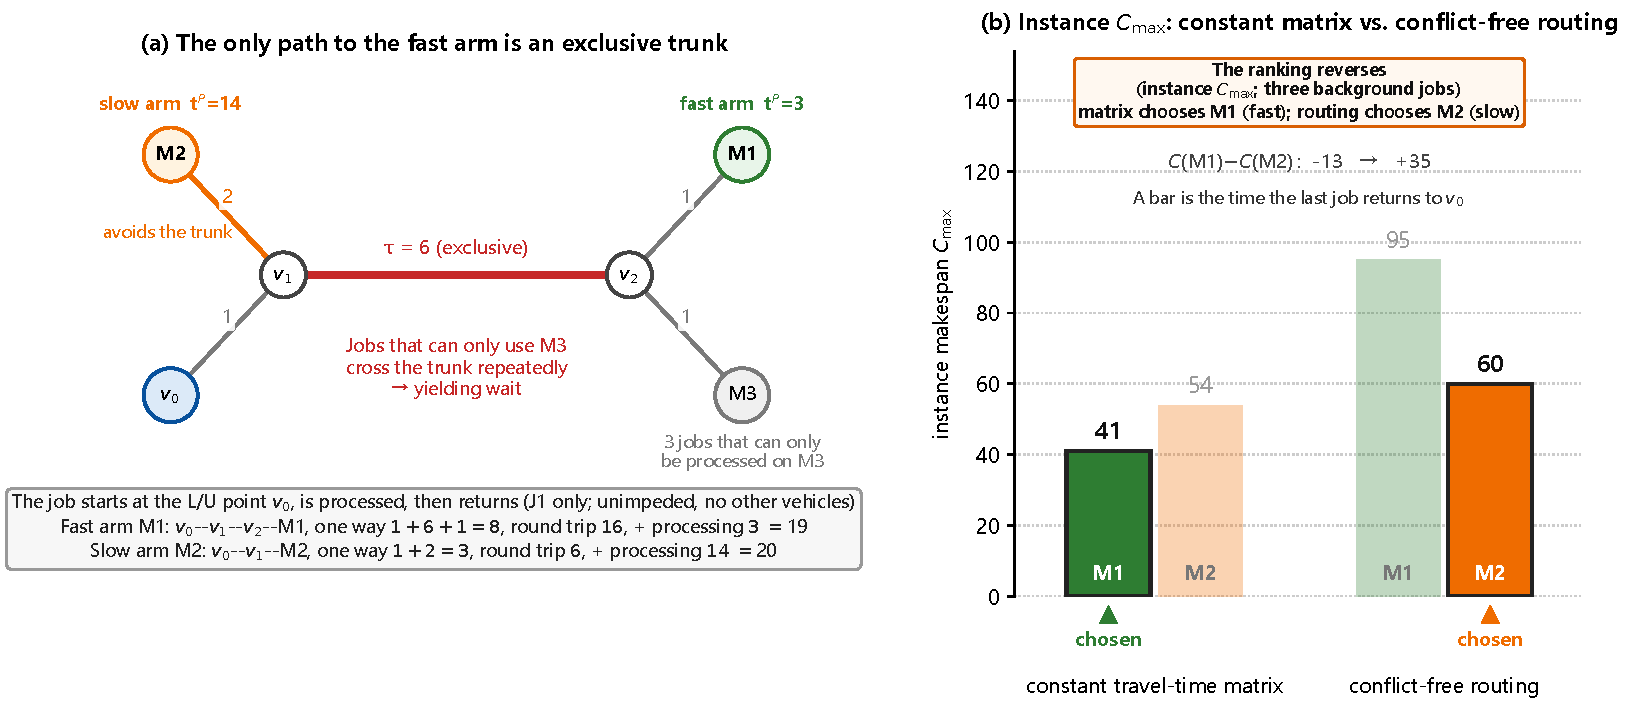
\includegraphics[width=\textwidth]{fig/fig_motivating.pdf}
\Description{Left: shop network with an exclusive trunk to the fast arm. Right: makespans of two assignments, 41 versus 54 under the constant matrix and 95 versus 60 under conflict-free routing.}
\caption{Motivating instance. (a)~Network: exclusive trunk ($\tau=6$) to the fast arm M1, short corridor to the slow arm M2, three M3-only jobs crossing the trunk. (b)~Instance makespan $C_{\max}$ of the two assignments of J1 under the constant matrix and under conflict-free routing. Of $1200$ nearby parameter combinations, $205$ ($17\%$) show the reversal.}
\label{fig:motivating}
%% Generated by fig/fig_motivating.py from clbs/output/motivating.json (same decoder as the paper).
\end{figure*}

Most existing work covers only part of this setting: scheduling with transportation uses a constant matrix, and conflict-free path planning takes task origins, destinations and release times as given.
Van Os and Basten~\cite{vanos2026exact} formalize the combined problem and solve small benchmark instances to proven optimality.
We focus on settings not previously taken as a dedicated object of study: transport longer than processing ($\bar{T}_t/\bar{T}_p\approx4.0$, against at most \PubTtTpHi{} on common public instances), corridors exclusive over their whole length (van Os and Basten reserve nodes; Section~\ref{sec:fjsppt}), waiting only at berths, and congestion on a few shared corridors, with contention intensity as a controlled variable and sizes that exact decomposition has difficulty solving.
There, heuristics schedule first and resolve conflicts afterwards~\cite{sun2023integrated}, feed back realized durations once without reassignment~\cite{li2026framework}, or embed routing in decoding without measuring its benefit and cost~\cite{lyu2019approach}.
Under equal compute it is thus unmeasured how to trade off ``fast but congested'' against ``slow but clear'' arms, what counting yielding delay in the search gains, and at what contention this gain is worth its cost.

\subsection{Approach and contributions}

The upper level of our closed-loop bilevel framework decides machine assignment and operation sequencing; the lower level plans conflict-free paths by time-window reservation.
On the evaluation path, routing-in-the-loop evaluation ranks each candidate by its makespan after conflict-free routing, so yielding wait enters the search objective; such a decode costs over an order of magnitude more than one on unimpeded times, and neither Li et al.~\cite{li2026framework}, who list a fully iterative loop as future work, nor Lyu et al.\ report its cost or gain.
On the decision path, reservation-table-aware dispatching trial-queries both legs for each candidate vehicle on the current reservation table, without writing it, and selects the earliest feasible delivery instead of idle-first dispatching~\cite{lu2022agv}; admissible lower-bound pruning and winner-path reuse skip only trial queries that cannot affect the result.

A four-level baseline ladder forms a $2\times2$ design over whether the search counts conflict-induced delay and whether vehicles are chosen by unimpeded time or by trial query: B0 is the open-loop structure of constant-matrix methods and Li et al.\ on a real network, B0+ dispatches by the reservation table on a frozen schedule as in Sun et al., B1 closes the loop with rule-based dispatching, and B2 is our method.
All share the search, the router and the wall-clock budget, and are compared by realized makespan (Section~\ref{sec:protocol}).
With dispatching fixed, the closed loop reduces makespan by \GainLoopRule{} ($p\PLoopRule$) and remains significant on \CellsSigLoopAdj{} of the \NCases{} instances after Holm correction; within it, reservation-table-aware dispatching adds \GainProbeLoop{} ($p\PProbeLoop$) but is significant on no single instance; end to end, the reduction is \GainEndToEnd{} ($p\PEndToEnd$), slightly below the \GainIndepProduct{} predicted by independent composition (Section~\ref{sec:main}).
Our contributions are:

\begin{enumerate}[leftmargin=*]
\item \textbf{Controlled instances.} Instance families with controllable contention intensity let us examine how high contention must be before counting yielding wait in the schedule brings a gain (Section~\ref{sec:instances}).
\item \textbf{Routing-in-the-loop evaluation.} Its gain and cost over the open loop are measured at an equal wall-clock budget, and every chromosome decodes into a conflict-free, deadlock-free timetable without repair (Proposition~\ref{prop:decodable}).
\item \textbf{Low-overhead dispatching.} The speed-ups make each dispatching evaluation \SpeedupProbe{} times faster without changing the selected vehicle or the final timetable (Proposition~\ref{prop:speedup_equiv}), which makes a net gain possible at an equal budget.
\item \textbf{Decomposed evidence.} The closed loop is the larger effect and dispatching a much smaller one whose sign varies with the vehicle-to-arm ratio; the two do not amplify each other. An extra cost on occupied corridor--time slots (hereafter, surcharge) and yield-record-guided reassignment or staggering only add overhead; the failure of the surcharge suggests checking first whether the receiving level's objective already contains what an interface would pass.
\end{enumerate}

Sections~\ref{sec:Chapter_II}--\ref{sec:Chapter_V} cover related work, the problem (notation in Table~\ref{tab:notation}), the framework and the experiments; the final section concludes.


\section{Related work}
\label{sec:Chapter_II}

Related work comprises scheduling with transportation, conflict-free routing with exogenous tasks, and their integration; Table~\ref{tab:related} compares them with this paper.

\subsection{Two strands}

Flexible job shop scheduling with transportation (FJSP\_PT) brings material movement into the schedule (FJSP review~\cite{dauzereperes2024fjsp}; benchmarks~\cite{homayouni2021production}), and its dominant convention is a constant travel-time matrix, a fixed $t(a,b)$ regardless of corridor occupancy~\cite{xin2025review}.
Recent work keeps the matrix and improves solution methods: Meng et al.~\cite{meng2025cp} close 29 open benchmark instances and improve 27 best-known solutions with constraint programming and a genetic algorithm; Qin et al.~\cite{qin2026knowledge} use Q-learning and a local search guided by AGVs and the critical path; Fu et al.~\cite{fu2025integrated} decide production and logistics jointly.
Vehicles thus never delay one another, and although critical-chain local search is mature~\cite{otala2021graph,tamssaouet2023neighborhood}, a critical path on the matrix leads back to an operation or a machine, not to a corridor; Xin et al.\ note that such assumptions ``even change [the problem's] nature'' and that $\bar{T}_t/\bar{T}_p$ is likely to affect algorithm performance.
% [ref_check: key=meng2025cp; claim="closes 29 open instances, improves 27 best-known solutions"; need=quote]

Optimal multi-agent path finding (MAPF) is NP-hard~\cite{gao2023mapf}, and Kasaura et al.~\cite{kasaura2022sipp} extend Safe Interval Path Planning to continuous-time road networks.
For continuously arriving tasks, Zhang et al.~\cite{zhang2024guidance} optimize edge weights offline to steer agents away from bottlenecks, and Kim and Kim~\cite{kim2026congestion} propose congestion-aware dispatching rules for large AGV fleets; surveys~\cite{lu2022agv,fragapane2021planning} treat dispatching and path planning as separate layers.
Task release times and endpoints are inputs, so the router cannot revise the assignment, and congestion is measured indirectly (local density, offline edge weights), without identifying which transport caused yielding, when, and where.

\subsection{Integration and our position}

Van Os and Basten~\cite{vanos2026exact} use logic-based Benders decomposition, whose integer-programming routing subproblem returns conflicts to a constraint-programming master as cuts; they solve most benchmarks to proven optimality and improve about half by at least 10\% over prior heuristics, but only at small scale, and list fuller use of ``which conflicts caused the infeasibility'' as future work.
Sun et al.~\cite{sun2023integrated} fix the schedule by a hybrid genetic algorithm and then resolve conflicts by time-window Dijkstra, so congestion found later cannot change the schedule.
Li et al.~\cite{li2026framework} feed realized durations back once, shifting start times of the current solution without reassignment, with one eligible machine per operation.
Lyu et al.~\cite{lyu2019approach} route inside genetic-algorithm decoding but study fleet sizing on small instances, with neither an open-loop comparison nor a cost report.

The gap is thus not whether conflicts are handled but how routing results enter the schedule and what that is worth.
Beyond the reach of exact decomposition, and with corridors rather than nodes reserved, we route every candidate, dispatch by trial query, measure both contributions at an equal wall-clock budget, and vary contention intensity, since instances with the same $\bar{T}_t/\bar{T}_p$ may differ greatly in how much congestion reassignment can bypass.

\begin{table}[t]
  \caption{Related work versus this paper. Het.: machine-dependent processing times on optional machines; Excl.: one vehicle per corridor at a time; transport times are unimpeded (ignoring other vehicles) or routed (with yielding wait). Controls: Section~\ref{sec:pricing}.}
\label{tab:related}
%% Hand-maintained table: any row change must match Section 2.2.
\footnotesize
\renewcommand{\arraystretch}{1.2}
\begin{tabular}{@{}p{2.5cm}cccp{2.9cm}p{3.1cm}@{}}
\toprule
Work class & Ref. & Het. & Excl. & Transport times used to evaluate schedules & Research focus \\
\midrule
FJSP\_PT metaheuristics & \cite{meng2025cp,qin2026knowledge,fu2025integrated} & yes & no & unimpeded (matrix) & quality under a matrix \\
Lifelong MAPF & \cite{gao2023mapf,zhang2024guidance} & --- & yes & none (tasks exogenous) & throughput \\
Congestion-aware dispatching & \cite{kim2026congestion} & --- & no & none (tasks exogenous) & large-fleet congestion \\
Two-stage FJSP + routing & \cite{sun2023integrated} & yes & yes & unimpeded; routed after freezing & schedule, then resolve \\
RL scheduling + PBS & \cite{li2026framework} & no & yes & unimpeded; one correction & RL with multi-vehicle paths \\
GA + time-window routing & \cite{lyu2019approach} & yes & yes & routed, every candidate & fleet size \\
Exact LBBD & \cite{vanos2026exact} & yes & no & bound + conflict cuts & small-scale optimality \\
\textbf{This paper} & & yes & yes & routed, every candidate; trial-query dispatching & fast/slow-arm trade-off; closed-loop gain and cost \\
\bottomrule
\end{tabular}
\end{table}
